\documentclass[11pt,letterpaper]{article}
\usepackage[utf8]{inputenc}
\usepackage[T1]{fontenc}
\usepackage[spanish,es-noshorthands,es-tabla]{babel}
\usepackage[margin=2.5cm]{geometry}
\usepackage{lmodern}
\usepackage{amsmath,amssymb}
\usepackage{graphicx}
\usepackage{booktabs}
\usepackage{caption}
\usepackage{enumitem}
\usepackage[hidelinks]{hyperref}
\captionsetup{font=small,labelfont=bf}
\setlength{\parskip}{3pt}
\setlist{itemsep=1pt,topsep=2pt}

\title{\vspace{-1.2cm}Agente de búsqueda heurística para Snake\\
\large Representación y solución automática de problemas}
\author{Daniel José Morales \and Juan Esteban Torres\\
\small Escuela de Ingeniería, Ciencia y Tecnología, Universidad del Rosario}
\date{}

\begin{document}
\maketitle
\vspace{-0.8cm}

% ============================================================
\section{Descripción del entorno}

El juego que decidimos desarrollar fue Snake, que se juega en una cuadrícula de $10 \times 10$ con celdas $(x, y) \in \{0, \dots, 9\}^2$. A simple vista el escenario es estocástico, porque el agente no sabe dónde aparecerá la siguiente fruta hasta comerse la actual. Sin embargo, una vez aparece la nueva fruta, el problema se vuelve determinista. Por eso descomponemos la partida en una secuencia de subproblemas deterministas que resuelve un agente basado en modelo y basado en objetivos.

\begin{table}[h]
\centering
\small
\caption{Caracterización del entorno.}
\label{tab:caracterizacion}
\begin{tabular}{ll}
\toprule
$\checkmark$ Completamente observable & \phantom{$\checkmark$} Parcialmente observable\\
$\checkmark$ Single-agent (Base) & $\checkmark$ Multi-agent (Variante)\\
$\checkmark$ Determinista (Micro) & $\checkmark$ Estocástico (Macro)\\
\phantom{$\checkmark$} Episódico & $\checkmark$ Secuencial\\
$\checkmark$ Estático (Por turnos) & \phantom{$\checkmark$} Dinámico\\
$\checkmark$ Discreto & \phantom{$\checkmark$} Continuo\\
$\checkmark$ Conocido (\emph{Model-Based}) & \phantom{$\checkmark$} Desconocido (\emph{Model-Free})\\
\bottomrule
\end{tabular}
\end{table}

\subsection*{Estados ($S$)}
En cada instante de tiempo $t$, el estado del entorno está definido por la tupla $s = (C, f)$, donde $C = (c_1, c_2, \dots, c_L)$ es la secuencia ordenada de coordenadas $(x, y) \in \{0, \dots, N-1\}^2$ que representan el cuerpo de la serpiente con $c_1$ como la cabeza, $c_L$ la cola y una longitud definida como $L = |C|$. $f \in \{0, \dots, N-1\}^2 \setminus C$ es la posición de la fruta actual. En las variantes con obstáculos fijos, la fruta tampoco puede aparecer sobre ellos.

\subsection*{Acciones ($A$)}
El conjunto de decisiones posibles lo definimos como: $\mathcal{A} = \{\text{norte}, \text{sur}, \text{este}, \text{oeste}\}$, con vectores de desplazamiento $\delta(a) \in \{(0,1), (0,-1), (1,0), (-1,0)\}$. Una acción $a \in \mathcal{A}$ es aplicable en el estado $s$ si la nueva posición de la cabeza $h' = c_1 + \delta(a)$ permanece dentro de los límites del tablero (o se envuelve modularmente en la variante toroidal) y no colisiona con los segmentos $c_1, \dots, c_{L-1}$ ni con obstáculos. La casilla de la cola $c_L$ sí es válida para $L > 2$ porque se desplaza en el mismo turno, y para $L \ge 2$ se excluye el giro de $180^\circ$ hacia el cuello $c_2$, dejando un factor de ramificación máximo $b \le 3$.

\subsection*{Función de recompensa ($R$)}
\emph{Costo / Pérdida de transición (Nivel Micro):} Cada movimiento en el árbol de búsqueda tiene un costo positivo que penaliza tanto el número de pasos como el riesgo de encierro local alrededor de la nueva cabeza $h'$:
\[
c(s, a, s') = 1 + \lambda \cdot r(h'), \qquad r(h') = \frac{\text{vecinos bloqueados}(h')}{3} \in [0, 1]
\]
donde $\text{vecinos bloqueados}(h') \in \{0, 1, 2, 3\}$ cuenta cuántas de las 3 direcciones futuras desde $h'$ están obstruidas por el cuerpo, muros o bordes del tablero, y $\lambda \ge 0$ pondera la aversión al riesgo.

\emph{Señal de Recompensa Inmediata y Acumulada (Nivel Macro):} En cada turno de la partida el entorno entrega una recompensa inmediata $R(s, a, s')$ definida por el balance entre ganancias y pérdidas:
\[
R(s, a, s') = \begin{cases}
+1000 - c(s,a,s') & \text{si } h' = f \text{ y } L' = N^2 - |\text{obstáculos}|, \text{ victoria} \\
+100 - c(s,a,s') & \text{si } h' = f \text{ y } L' < N^2 - |\text{obstáculos}|, \text{ fruta comida} \\
-100 - c(s,a,s') & \text{si } s' \text{ queda sin acciones aplicables, derrota} \\
-100 - c(s,a,s') & \text{si se completan } k_{\max} \text{ pasos sin comer} \\
-c(s,a,s') & \text{en un desplazamiento normal, } h' \neq f
\end{cases}
\]
La \textbf{recompensa acumulada} a lo largo del episodio ($G = \sum_{t} R_t$) se relaciona directamente con los objetivos del proyecto: maximizar $G$ exige maximizar el número de frutas consumidas mientras se minimiza la cantidad de pasos y el riesgo de auto-encierro.

\subsection*{Función de transición ($T$)}
Dada una acción aplicable $a$ que lleva la cabeza a $h' = c_1 + \delta(a)$, el entorno evoluciona mediante dos casos:
\begin{enumerate}
  \item \emph{Desplazamiento sin comer ($h' \neq f$):} El cuerpo avanza una celda y la cola libera su casilla anterior, resultando en $C' = (h', c_1, \dots, c_{L-1})$ con la misma fruta $f' = f$.
  \item \emph{Crecimiento al comer ($h' = f$):} La serpiente incrementa su longitud en una unidad sin desplazar la cola, resultando en $C' = (h', c_1, \dots, c_L)$, y aparece una nueva fruta $f'$ elegida con distribución aleatoria uniforme entre las celdas libres (o colocada por el oponente Minimax en la variante adversaria).
\end{enumerate}
La dinámica física del cuerpo es \textbf{completamente conocida (\emph{Model-Based})}, lo que permite al agente simular trayectorias exactas durante la planeación.

\subsection*{Objetivo y estados terminales}
\begin{itemize}
  \item \emph{Objetivo por subproblema (Micro):} Encontrar un camino de acciones que lleve la cabeza hasta la fruta actual ($c_1 = f$) minimizando el costo acumulado $g(n) = \sum c(s_i, a_i, s_{i+1})$, sujeto a la restricción de seguridad de que en el estado final simulado exista al menos una ruta válida desde la cabeza hasta la cola $c_L$.
  \item \emph{Objetivo global (Macro):} Maximizar la longitud final alcanzada $L_{\text{final}}$ (y la recompensa acumulada $G$) hasta lograr llenar el tablero.
  \item \emph{Estados terminales:} Un episodio termina cuando se alcanza cualquiera de los siguientes tres estados: \textbf{(1) Victoria}, al llenar todas las celdas disponibles del tablero ($L = 100$ en la versión base $10\times 10$); \textbf{(2) Encierro o colisión}, cuando desde el estado actual no existe ninguna acción aplicable ($\mathcal{A}(s) = \emptyset$); o \textbf{(3) Límite de pasos sin comer}, cuando transcurren $k_{\max} = 200$ turnos consecutivos sin consumir una fruta.
\end{itemize}

\subsection*{Variantes de complejidad creciente}
\begin{enumerate}
  \item \textbf{Tablero Toroidal (sin bordes):} La distancia Manhattan clásica deja de ser admisible y el agente emplea la distancia Manhattan toroidal $\min(|\Delta x|, N-|\Delta x|) + \min(|\Delta y|, N-|\Delta y|)$.
  \item \textbf{Múltiples frutas simultáneas (3 frutas) + Obstáculos fijos:} El agente toma $h(s) = \min_{i} d(c_1, f_i)$ sorteando muros estáticos en un tablero $12 \times 12$.
  \item \textbf{Fruta Adversaria (Minimax con Poda Alfa-Beta):} Un segundo jugador (\texttt{AgenteFruta\allowbreak Adversaria}) coloca cada nueva fruta en la celda libre que minimiza la utilidad esperada de la serpiente.
\end{enumerate}

% ============================================================
\section{Tipo de agente y justificación}

Nuestro agente, \texttt{AgenteSnake}, es un agente basado en modelo y basado en objetivos. Es basado en modelo porque conoce exactamente cómo se mueve el cuerpo de la serpiente, así que puede simular qué pasaría si sigue un camino antes de moverse. Es basado en objetivos porque cada vez que aparece una fruta se plantea una meta concreta, que es llevar la cabeza hasta esa casilla, y busca una secuencia de acciones que la cumpla.

Elegimos este tipo de agente porque encaja con la forma del problema. Mientras una fruta está en el tablero no hay nada aleatorio, de modo que planear todo el camino de una vez es razonable. La incertidumbre solo aparece cuando la fruta se come y surge otra en una casilla al azar. Por eso el agente trabaja por ciclos: planea un camino hasta la fruta actual, lo ejecuta paso a paso y vuelve a planear cuando cambia la fruta o cuando la siguiente acción del plan deja de ser aplicable. Un agente reactivo simple no serviría, porque mirando solo las casillas vecinas no puede anticipar que un camino corto lo va a dejar encerrado diez pasos después.

La parte más importante del agente es el chequeo de seguridad. Antes de comprometerse con un camino, el agente toma el estado en el que quedaría justo después de comer y resuelve un segundo problema de búsqueda con BFS, esta vez desde la cabeza hasta su propia cola $c_L$. La idea es que si la cabeza todavía puede alcanzar la cola, la serpiente siempre tiene una salida, porque la cola va liberando casillas a medida que avanza. Si ese camino existe, el agente ejecuta el plan completo. Si no existe, o si ni siquiera hay camino hasta la fruta, el agente no se arriesga y da un solo paso de evasión. Para elegirlo prueba cada acción aplicable, se queda con las que mantienen un camino hasta la cola y entre ellas prefiere la que deja la cola más lejos, tiene menos vecinos bloqueados y se acerca un poco a la fruta. Después de ese paso vuelve a planear desde cero.

% ============================================================
\section{Algoritmos implementados}

Todos los algoritmos están en \texttt{busqueda.py} y son versiones en grafo de los vistos en clase. Cada uno lleva una lista de estados explorados para no expandir dos veces el mismo estado. Para que esa lista sea pequeña, la función \texttt{codigo} identifica un estado solo por la casilla de la cabeza. Es una simplificación consciente. Dentro de un mismo subproblema el cuerpo cambia poco entre caminos alternativos, y así el espacio de búsqueda queda acotado por las $N^2 = 100$ casillas del tablero. A cambio, en casos raros la búsqueda puede descartar un camino válido que llega a una casilla ya visitada con el cuerpo en otra posición.

\begin{itemize}
  \item \textbf{Anchura, BFS.} Expande por niveles con una cola FIFO. Encuentra el camino con menos pasos, que coincide con el de menor costo solo cuando $\lambda = 0$.
  \item \textbf{Profundidad, DFS.} Usa una pila y sigue una rama hasta el fondo antes de retroceder. Siempre encuentra un camino si existe, pero suele ser muy largo. Lo incluimos como punto de contraste.
  \item \textbf{Costo uniforme, Dijkstra.} Expande el nodo con menor $g(n)$. Con $\lambda > 0$ es el único algoritmo ciego que respeta el costo por riesgo.
  \item \textbf{Avara.} Ordena la frontera solo por $h(n)$. Es la más rápida, pero puede preferir un camino que parece corto y no lo es.
  \item \textbf{A$^*$.} Ordena por $f(n) = g(n) + h(n)$. Con una heurística admisible devuelve el camino de menor costo y expande menos nodos que Dijkstra.
  \item \textbf{Haz con $k = 3$.} Igual que A$^*$, pero en cada iteración conserva solo los $k$ mejores nodos de la frontera. Usa muy poca memoria, aunque puede podar justo el nodo que llevaba a la solución.
\end{itemize}

En la Tabla~\ref{tab:algoritmos}, $b \le 3$ es el factor de ramificación, $d$ la profundidad de la solución más corta, $m$ la profundidad máxima del grafo, $C^*$ el costo óptimo y $\varepsilon = 1$ el costo mínimo de un paso. Como el grafo tiene a lo sumo $N^2$ nodos, en la práctica todas estas cotas quedan limitadas por $O(N^2)$.

\begin{table}[h]
\centering
\small
\caption{Propiedades de los algoritmos en el subproblema de llegar a la fruta.}
\label{tab:algoritmos}
\begin{tabular}{lcccc}
\toprule
Algoritmo & Completo & Óptimo & Tiempo & Espacio\\
\midrule
BFS (anchura)       & Sí & Solo si $\lambda = 0$ & $O(b^d)$ & $O(b^d)$\\
DFS (profundidad)   & Sí, grafo finito & No & $O(b^m)$ & $O(bm)$\\
UCS (Dijkstra)      & Sí & Sí & $O(b^{1+\lfloor C^*/\varepsilon \rfloor})$ & $O(b^{1+\lfloor C^*/\varepsilon \rfloor})$\\
Avara               & Sí, grafo finito & No & $O(b^m)$ & $O(b^m)$\\
A$^*$               & Sí & Sí, con $h$ admisible & $O(b^d)$ & $O(b^d)$\\
Haz ($k=3$)         & No & No & $O(k\,b\,m)$ & $O(k)$\\
\bottomrule
\end{tabular}
\end{table}

\subsection*{Heurísticas}
Implementamos tres heurísticas. La primera, $h_1$, es la distancia Manhattan entre la cabeza y la fruta. La segunda, $h_2$, es la distancia euclídea. La tercera, $h_3 = h_1 + 2\,r(c_1)$, suma a la Manhattan una penalización por los vecinos bloqueados alrededor de la cabeza.

$h_1$ es admisible porque cada movimiento cambia la cabeza en una sola casilla y cuesta al menos 1, así que nunca se llega a la fruta con un costo menor que la distancia Manhattan. También es consistente, ya que entre dos estados vecinos su valor cambia como mucho en 1. $h_2$ es menor o igual que $h_1$, por lo que también es admisible, pero informa menos. $h_3$ no es admisible, porque la penalización puede sumar hasta 2 unidades que el camino real no paga. En la Sección~3.3 del notebook lo comprobamos sobre 30 estados de una partida real, comparando cada heurística con el costo óptimo calculado con Dijkstra. $h_1$ y $h_2$ fueron admisibles en todos los estados y $h_3$ solo en el 73\,\%. Aun así, en esa muestra A$^*$ encontró el óptimo con las tres, y $h_3$ expandió en promedio 10.8 nodos frente a 10.9 de $h_1$ y 12.2 de $h_2$.

\subsection*{Comparación en una instancia}
En la Sección~3.2 del notebook corrimos los seis algoritmos sobre una misma instancia con 8 obstáculos y $\lambda = 0.5$. Todos encontraron la fruta. BFS llegó en 8 pasos pero con costo 8.67, mayor que el óptimo de 8.33, porque cuenta pasos y no riesgo. DFS dio un camino de 20 pasos y expandió 87 nodos. Dijkstra encontró el óptimo expandiendo 78 nodos y A$^*$ con $h_1$ lo encontró expandiendo 20. La avara con $h_1$ expandió solo 9 pero no llegó al óptimo, y el haz sí llegó con 14 nodos expandidos y una frontera de apenas 3.

% ============================================================
\section{Diseño experimental, resultados y análisis}

Para comparar los algoritmos jugamos partidas completas sobre las semillas 0 a 99, de modo que cada configuración enfrenta exactamente las mismas secuencias de frutas. Todas las partidas usan un tablero de $10 \times 10$ sin obstáculos, la cabeza empieza en $(5,5)$, $k_{\max} = 200$ y cada partida se corta a los 2500 pasos si no ha terminado. Evaluamos los seis algoritmos con y sin chequeo de seguridad. Con chequeo agregamos además A$^*$ con $h_2$ y A$^*$ con $\lambda = 0.5$, para ver el efecto de la heurística y del costo por riesgo. Dijkstra se corre siempre con $\lambda = 0.5$, porque con $\lambda = 0$ se comporta igual que BFS. En total son 14 configuraciones y 1400 partidas, guardadas en \texttt{resultados\_benchmark\_100\_semillas.csv}. De cada partida registramos la longitud final, si hubo victoria, la causa de fin, los pasos por fruta y, para cada decisión, los nodos generados y expandidos, la frontera máxima y el tiempo.

\begin{table}[!htb]
\centering
\footnotesize
\setlength{\tabcolsep}{4pt}
\caption{Resultados promedio sobre 100 semillas (0--99), tablero $10\times10$, $k_{\max}=200$. Nodos y frontera son promedios por decisión.}
\label{tab:resultados}
\begin{tabular}{lcccccrrrr}
\toprule
Algoritmo & $\lambda$ & Long. final & Vict. (\%) & Fin $k_{\max}$ (\%) & Pasos/fruta & Gen. & Exp. & Front. máx. & $t$ (ms)\\
\midrule
\multicolumn{10}{l}{\textit{Sin chequeo de seguridad}}\\
BFS & 0.0 & 34.2 $\pm$ 8.3 & 0 & 0 & 8.0 & 44.3 & 37.4 & 18.1 & 0.88\\
DFS & 0.0 & 23.0 $\pm$ 1.8 & 0 & 0 & 40.5 & 82.8 & 46.5 & 77.0 & 1.05\\
UCS & 0.5 & 32.1 $\pm$ 7.8 & 0 & 0 & 7.8 & 52.0 & 44.9 & 21.1 & 1.77\\
Avara (Manh.) & 0.0 & 34.1 $\pm$ 8.6 & 0 & 0 & 8.2 & 21.7 & 12.8 & 23.4 & 0.97\\
A* (Manh.) & 0.0 & 34.9 $\pm$ 9.1 & 0 & 0 & 8.1 & 29.2 & 20.7 & 22.3 & 0.97\\
Haz (Manh.) & 0.0 & 34.7 $\pm$ 9.7 & 0 & 0 & 8.3 & 26.1 & 16.1 & 7.0 & 0.71\\
\midrule
\multicolumn{10}{l}{\textit{Con chequeo de seguridad}}\\
BFS & 0.0 & 91.5 $\pm$ 12.1 & 8 & 82 & 19.1 & 57.3 & 50.7 & 18.3 & 1.09\\
DFS & 0.0 & 94.4 $\pm$ 13.1 & 75 & 0 & 25.1 & 177.2 & 124.6 & 80.9 & 2.56\\
UCS & 0.5 & 91.4 $\pm$ 6.7 & 0 & 90 & 20.9 & 58.8 & 53.2 & 21.1 & 2.02\\
Avara (Manh.) & 0.0 & 93.5 $\pm$ 9.4 & 7 & 89 & 20.0 & 52.0 & 43.8 & 24.1 & 1.73\\
A* (Manh.) & 0.0 & 93.3 $\pm$ 8.5 & 2 & 92 & 20.3 & 54.6 & 47.9 & 22.7 & 1.89\\
A* (Eucl.) & 0.0 & 93.1 $\pm$ 7.6 & 3 & 92 & 20.8 & 53.6 & 47.2 & 24.8 & 1.90\\
A* (Manh.) & 0.5 & 91.0 $\pm$ 7.2 & 2 & 92 & 20.7 & 54.6 & 46.9 & 26.6 & 2.71\\
Haz (Manh.) & 0.0 & 92.3 $\pm$ 8.8 & 1 & 89 & 20.1 & 51.1 & 42.3 & 16.5 & 1.62\\
\bottomrule
\end{tabular}
\end{table}


\begin{figure}[!htb]
\centering
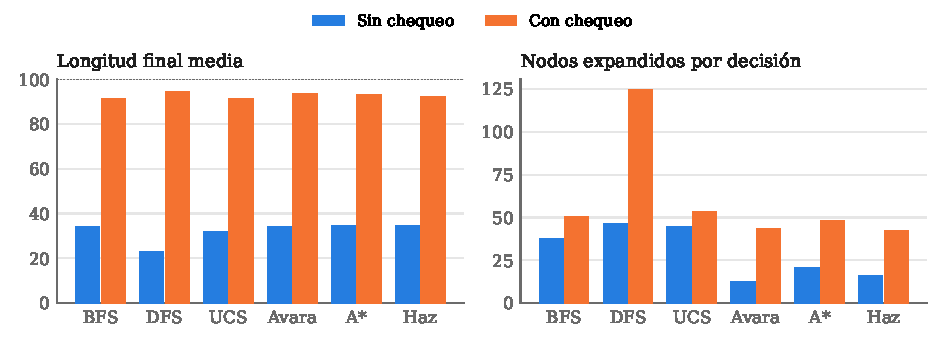
\includegraphics[width=\linewidth]{fig_resultados.pdf}
\caption{Longitud final media y nodos expandidos por decisión con y sin chequeo de seguridad. Se usa $\lambda=0$ salvo en UCS, que usa $\lambda=0.5$. La línea punteada marca el tablero lleno.}
\label{fig:resultados}
\end{figure}

\subsection*{El chequeo de seguridad es lo que más importa}
El resultado más claro de la Tabla~\ref{tab:resultados} es que el chequeo de seguridad pesa mucho más que el algoritmo elegido. Sin él, las 600 partidas terminaron con la serpiente encerrada, y BFS, Dijkstra, la avara, A$^*$ y el haz quedaron todos entre 32 y 35 de longitud. Ir siempre por el camino más corto funciona al principio, pero cuando el cuerpo pasa de unas 30 casillas la serpiente termina metiéndose en una zona sin salida. Con el chequeo, la longitud media sube a valores entre 91 y 94 y los encierros bajan a entre 2 y 10 partidas de cada 100.

El costo de esa seguridad se ve en dos lugares. Los pasos por fruta pasan de unos 8 a unos 20, porque el agente a veces rodea o sigue su cola en vez de ir directo. Además, cada decisión expande más nodos, ya que aparte de buscar la fruta hay que resolver la búsqueda hasta la cola. Aun así, ninguna configuración tarda en promedio más de 3 ms por decisión.

\subsection*{Por qué casi no hay victorias}
Con chequeo, la mayoría de las partidas no termina por choque sino por llegar a $k_{\max}$, entre el 82\,\% y el 92\,\% según el algoritmo. Cuando la serpiente ya ocupa más de 90 casillas, casi cualquier camino hacia la fruta la dejaría sin salida, así que el agente se queda dando pasos de evasión detrás de su cola. Eso la mantiene viva, pero entra en un ciclo y no vuelve a comer. El chequeo evita perder, pero por sí solo no basta para ganar.

La excepción es DFS, que ganó 75 de las 100 partidas. Su forma de explorar produce caminos largos que barren el tablero casi fila por fila, y ese recorrido deja el cuerpo ordenado y con espacio libre detrás. Sin chequeo ese mismo comportamiento es el peor, con 23 de longitud y 40 pasos por fruta. Hay que tener en cuenta que 23 de sus partidas con chequeo llegaron al tope de 2500 pasos sin terminar, así que su longitud media está algo subestimada. También es la configuración más cara, con 124.6 nodos expandidos por decisión.

\subsection*{Heurísticas y costo por riesgo}
Sin chequeo, la avara expandió 12.8 nodos por decisión, el haz 16.1 y A$^*$ 20.7, frente a 37.4 de BFS y 44.9 de Dijkstra, sin perder longitud. Con chequeo esas diferencias casi desaparecen, porque la búsqueda hasta la cola, que siempre se hace con BFS, pasa a ser la parte más costosa de cada decisión. Cambiar $h_1$ por $h_2$ en A$^*$ no cambió nada importante: 93.3 contra 93.1 de longitud y prácticamente los mismos nodos. Usar $\lambda = 0.5$ tampoco ayudó. A$^*$ bajó de 93.3 a 91.0 y su tiempo por decisión subió de 1.89 a 2.71 ms. El costo por riesgo solo mira las casillas vecinas de la cabeza, y eso es demasiado local para prevenir los encierros, que se forman a la escala de todo el cuerpo. El chequeo de seguridad sí mira esa escala, y por eso es el que marca la diferencia.

% ============================================================
\section{Conclusiones}

Descomponer Snake en una secuencia de subproblemas deterministas funcionó bien. Cada subproblema se resuelve en milisegundos con cualquiera de los seis algoritmos, y como el agente conoce el modelo puede simular el resultado de un plan antes de ejecutarlo.

La conclusión principal es que buscar bien no alcanza si no se revisa a dónde lleva el camino. Sin el chequeo de seguridad todos los algoritmos se encierran alrededor de las 34 casillas. Con él, la serpiente llega en promedio a más de 90 de las 100. Frente a eso, las diferencias entre algoritmos y heurísticas son pequeñas. A$^*$ con $h_1$ sigue siendo la opción más equilibrada, porque es óptimo y expande pocos nodos. La avara y el haz son más baratos y en este problema casi no pierden calidad.

El punto débil del agente está al final de la partida. Con el tablero casi lleno prefiere seguir su cola antes que arriesgarse, y casi siempre termina por $k_{\max}$. El buen resultado de DFS sugiere que para ganar hace falta recorrer el tablero de forma más ordenada en la fase final, por ejemplo con un ciclo hamiltoniano, o aceptar caminos más largos que dejen espacio libre detrás. Ese sería el siguiente paso natural del proyecto, junto con medir de forma sistemática las tres variantes: el tablero toroidal, las tres frutas con obstáculos y la fruta adversaria con Minimax.

% ============================================================
\section{Declaración del uso de IA}
% Revisar y ajustar para que refleje exactamente cómo usaron la IA.
Usamos herramientas de IA generativa, según lo autorizado en las instrucciones del proyecto, en tres partes del trabajo. La primera fue el desarrollo de la aplicación gráfica SnakeLab Studio, es decir \texttt{interfaz.py} y la carpeta \texttt{web/}. La segunda fue la revisión del código y del notebook para encontrar errores y celdas incompletas. La tercera fue el apoyo en la redacción de algunas secciones de este informe a partir de nuestros resultados. El modelado del problema, el diseño del agente, los algoritmos y los experimentos son trabajo nuestro, y revisamos todo el texto y el código antes de entregarlo.

% ============================================================
\begin{thebibliography}{9}\small
\bibitem{aima} S.~Russell y P.~Norvig, \emph{Artificial Intelligence: A Modern Approach}, 4.\textsuperscript{a} ed. Pearson, 2021.
\end{thebibliography}

\end{document}
